\documentclass[10pt,twocolumn,letterpaper]{article}

% Classic conference format, reconstructed from the packages available in
% the lab image (the image ships no acmart/llncs/IEEEtran, and the hostile
% zone has no network so they cannot be fetched).

\usepackage[T1]{fontenc}
\usepackage{times}
\usepackage{amsmath,amssymb}
\usepackage{booktabs}
\usepackage{graphicx}
\usepackage[hidelinks]{hyperref}
\usepackage{microtype}
\usepackage{setspace}
\usepackage[letterpaper,top=1.0in,bottom=1.1in,left=0.75in,right=0.75in,columnsep=0.31in]{geometry}
\usepackage{caption}

\captionsetup{font=small,labelfont=bf}

\newcommand{\code}[1]{\texttt{#1}}
% break long identifiers without inserting a visible space
\newcommand{\bs}{\allowbreak\hspace{0pt}}
\setlength{\tabcolsep}{4.5pt}
\setlength{\parskip}{0pt}
\setstretch{1.02}

% ---- ACL-style title block inside a two-column document -------------------
\newcommand{\papertitle}{Provisional Constants: Disclosure and Calibration of\\
Decision Thresholds in a Self-Evaluating Research System}
\newcommand{\paperauthors}{
  \Large\textbf{An audit of the \code{labloop} agentic ML laboratory}\\[2pt]
  \normalsize
  \begin{tabular}{c}
  Prepared with \code{opencode}, operating the \code{labloop} MCP lab\\
  \small Reproduced against \code{github.com/cloudcell/labloop}, commit \code{21d91f1}
  \end{tabular}
}
\newcommand{\papermail}{\small Artifact identifiers appear in \S\ref{sec:artifacts}.}

\title{\papertitle}
\author{\paperauthors\\\papermail}
\date{}

\begin{document}
\maketitle

\begin{abstract}
Autonomous research systems increasingly make promotion decisions by comparing scalar scores.
We audit \code{labloop}, a five-server agentic ML laboratory in which an agent proposes meta-changes,
a \emph{tournament} compares the resulting improver against its own parent, and a \emph{campaign}
promotes a challenger over a champion. We find that the scalars driving these decisions are not
measurements. Using three complementary audits---provenance tracing, behavioural differential
testing, and Monte-Carlo benchmarking of the scoring function against known ground truth---we
establish four results. (i) A production confidence constant is traceable to a unit-test fixture
that asserted the value should be \emph{rejected}. (ii) The confidence recorded for a scientific
claim is a function of the verdict string alone: it does not vary across a 900-fold change in
measurement variance or a 45-fold change in effect size. (iii) The contract field designated as a
``pre-registered promotion policy'' is stored, frozen, displayed, and never read by any code path.
(iv) Under a true null, the tournament promotion signal exceeds 1.0 with probability $0.50$ at one
seed, and for a genuine small improvement it returns the wrong sign $37.8$ percent of the time.
We argue that a decision constant is not a parameter but a claim, and therefore requires a source;
we propose a \emph{provisional-constants protocol} that makes the absence of a source explicit in
the artifact rather than implicit in the diff.
\end{abstract}

\section{Introduction}
\label{sec:intro}

A research agent that runs its own experiments faces a problem that human laboratories solve with
social structure: who decides that one result is better than another, and on what grounds? Recent
systems answer by computing a scalar and comparing it to a threshold. \code{labloop} is such a
system. An agent registers an \emph{improver} version, submits a typed \emph{meta-change proposal},
and enters a \emph{tournament} in which a candidate improver is evaluated against its own parent
under a shared budget. If the tournament's \code{recursive\_gain} exceeds one, a descendant
\emph{campaign} may promote a challenger over the incumbent champion. Downstream, every hypothesis
verdict mints a \emph{claim} into a memory graph carrying a \code{confidence} scalar.

Every one of those numbers is presented to the operator in the grammar of measurement. They
appear in a status digest, in a web dashboard, in an MCP resource, as \code{float} fields in a
public API. Nothing in the interface distinguishes a number that was derived from data from one
that was typed into a source file by a maintainer at four in the morning.

We argue that this is the central failure mode of self-evaluating research systems, and that it
is not primarily a statistics problem. The arithmetic in \code{labloop} is, in the main, correct and
in one respect exemplary: the tournament score refuses to divide by zero. The problem is that
several of the system's numbers carry no information at all, and the interface does not say so.

This paper makes three contributions.

\begin{itemize}
\item \textbf{A taxonomy} of decision constants in self-evaluating research systems, separating
those that are epistemic claims about evidence from those that are operational parameters
(\S\ref{sec:taxonomy}). The distinction matters because only the former require a source.
\item \textbf{An audit method} comprising three cheap techniques---provenance tracing, behavioural
differential testing, and analytic benchmarking---that together localise a constant's origin and
measure its information content without requiring access to private design records
(\S\ref{sec:method}).
\item \textbf{An empirical case study} of \code{labloop} yielding four findings, including a
measured $37.8$ percent sign-error rate and an inert pre-registration mechanism
(\S\ref{sec:findings}).
\end{itemize}

We then set out \emph{best practice} for selecting each class of constant (\S\ref{sec:bestpractice})
and propose a \emph{provisional-constants protocol} (\S\ref{sec:protocol}) under which every
decision constant carries an explicit source status, and under which a value whose status is
\code{PROVISIONAL} may not be cited as grounds for a promotion decision.

The paper's thesis is stated plainly: \textbf{a decision constant is not a parameter, it is a
claim}. The difference is that a parameter may be tuned without anyone being misled, whereas a
claim, published without a source, is an assertion that has escaped scrutiny. The correct treatment
of an unsourced constant is not to delete it---many are load-bearing and the system genuinely needs
a value---but to \emph{label it} \code{PROVISIONAL} and to prevent decisions from resting on it
until it is sourced.

\section{The System Under Audit}
\label{sec:system}

\code{labloop} comprises five MCP servers implementing three nested loops. \emph{Loop 0}
(\code{episteme}) owns programmes, hypotheses, trials, observations, and conclusions. \emph{Loop 1}
(\code{zetesis}) owns investigations and champion/challenger promotion campaigns. \emph{Loop 2}
(\code{arete}) owns improver lineages, meta-change proposals, and paired ancestral tournaments. A
fifth server, \code{anamnesis}, is a claim graph; the fifth, \code{agora}, is a status hub.

Three quantities matter for this audit. All three are reproduced verbatim in \S\ref{sec:method}.

\paragraph{The tournament signal.} On closing a paired tournament, \code{arete} computes
\code{recursive\_gain} as the direction-normalised ratio of the per-seed best primary metric,
$E[\mathrm{best} \mid \mathrm{candidate}] / E[\mathrm{best} \mid \mathrm{parent}]$ for
$\mathrm{direction} = \mathrm{max}$, inverted for $\mathrm{direction} = \mathrm{min}$. If the
divisor arm's mean is exactly zero the close is \emph{refused} with a named, actionable error.

\paragraph{The campaign signal.} On closing a campaign, \code{zetesis} computes
\code{promotion\_score} as $\mathrm{mean}(\mathrm{challenger}) / \mathrm{mean}(\mathrm{champion})$.
If the champion mean is zero the score is set to $0.0$ and the campaign closes normally.

\paragraph{Claim confidence.} When a hypothesis concludes, \code{episteme} mints a claim with
\code{VERDICT\_CONFIDENCE[verdict]} --- literally $0.85$ for both \code{accepted} and
\code{rejected}. Independently, every \code{arete} meta-decision mints a claim at a hardcoded
$0.6$, and \code{anamnesis} and \code{zetesis} each define
\code{PRIOR\_CONFIDENCE\_MAX = 0.3}, an unstated ceiling on confidence for claims lacking an
evidence-bearing edge.

A promotion policy is a required, non-empty field on both contract types, documented as
``the pre-registered promotion rule (confidence bar, safety gates).'' It is versioned, frozen at
tournament open, and rendered in the dashboard. \code{S\ref{sec:findings}} reports what happens
next, which is nothing.

\section{A Taxonomy of Decision Constants}
\label{sec:taxonomy}

Not all magic numbers deserve equal scepticism. We classify the constants in a system such as this
into four classes, distinguished by the kind of warrant they require.

\paragraph{C1. Calibration constants.} Quantities that purport to summarise the strength of
evidence: confidences, priors, posteriors, credences. These are \emph{numerical claims about the
world} and are only meaningful relative to a model. \code{PRIOR\_CONFIDENCE\_MAX = 0.3} and
\code{VERDICT\_CONFIDENCE = 0.85} are C1. A C1 constant requires a derivation: from what prior,
under what likelihood, with what sample?

\paragraph{C2. Discriminative constants.} Thresholds and sample-size requirements that determine
whether a comparison is interpreted as a result: significance levels, minimum seed counts, minimum
detectable effects, comparison thresholds. These are C2 because they are choices about \emph{how
much evidence to require}, and such choices are only defensible relative to a stated cost of error
and a stated target effect. A C2 constant requires a power calculation.

\paragraph{C3. Governance constants.} Time limits after which an open record is considered
abandoned or a write is refused: staleness thresholds, freshness TTLs, decision-debt windows. These
encode a cost asymmetry (the cost of acting on a stale record versus the cost of waiting) and are
therefore C3, requiring that asymmetry to be stated even if no computation follows from it.

\paragraph{C4. Operational constants.} Timeouts, retention counts, pagination limits, bind
addresses. These are C4. They are genuinely operator knobs, they are honestly described as such,
and their correct value is a matter of preference rather than truth. Demanding a citation for
\code{DEFAULT\_LOG\_MAX\_FILES = 100} would be a category error.

The pragmatic value of the taxonomy is that it tells an auditor where to spend effort. C1 and C2
constants are where unsourced values do real damage, because they are consumed by a decision
procedure. C3 constants are where a quiet inconsistency between two servers causes an operational
incident. C4 constants are largely not the auditor's business. In \code{labloop}, a repository-wide
survey finds 41 module-level numeric constants and a large number of inline literals; the
distribution across classes is roughly $4$ C1, $6$ C2, $9$ C3, and the remainder C4.

\section{Method: Three Cheap Audits}
\label{sec:method}

The obstacle to auditing a self-evaluating system is that its design records are private. The
public repository is a squashed import of forty commits. We therefore rely on three techniques
that require no access to design history.

\subsection{P1. Provenance tracing}
\label{sec:p1}

Ask \code{git log -L} for the line that introduced the constant; then ask what the same literal
meant in the most recent commit before that. Constants frequently originate in test fixtures, where
they encode a \emph{rejection} condition, and are later copied into production paths where they
encode an \emph{assertion}. The semantic inversion is invisible at the call site and recoverable
only from history.

\subsection{P2. Behavioural differential testing}
\label{sec:p2}

Find two implementations of the same mathematical concept in one system and drive both with an
identical input. Divergence is a specification defect regardless of which branch is correct. This
technique requires no statistics and produces categorical results.

\subsection{P3. Analytic benchmarking against known ground truth}
\label{sec:p3}

Choose the ground truth rather than estimate it. The scoring function is a closed-form function of
recorded metrics, so it can be re-implemented verbatim and evaluated over a Monte-Carlo ensemble in
which the true effect is a chosen parameter. The re-implementation must then be \emph{calibrated}
against live observations to establish that it behaves as the server does. The benchmark itself
should run as a sealed trial in the audited system, so that its result enters the system of record
rather than a private notebook.

\section{Findings}
\label{sec:findings}

Figure~\ref{fig:flow} traces the derivation of every scoring value in the system, from the
hardcoded literal that seeds it to the surface on which an operator reads it. The figure is the
summary of this section; the subsections supply the evidence for each edge in it.

\begin{figure*}[t]
\centering
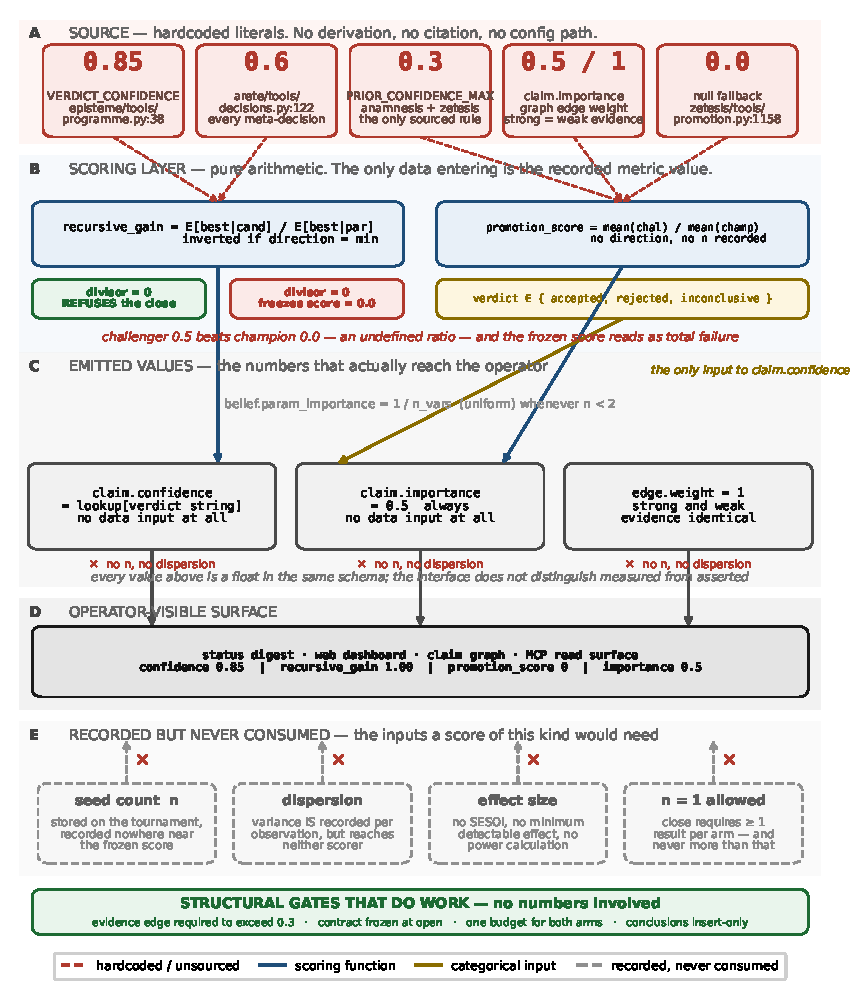
\includegraphics[width=\textwidth,height=0.92\textheight,keepaspectratio]{flow.pdf}
\caption{Derivation of the scoring values. \textbf{A}: the literals that seed every value below,
each carrying a file and line. \textbf{B}: the two scoring functions, which are pure arithmetic;
the only data entering them is the recorded metric value. The two green and red boxes show the
behavioural divergence of \S\ref{sec:f5} on an identical input. The gold box is the sole input to
\code{claim.confidence}. \textbf{C}: the emitted values. Every one is a \code{float} in the same
schema; the interface does not distinguish a value derived from data from a value typed into a
source file. \textbf{D}: the operator-visible surface. \textbf{E}: inputs the system records but
never consumes --- the seed count, the dispersion, and any statement of effect size --- with the
dashed arrows terminating in a cross. The green footer lists the structural gates that function
correctly and involve no numbers at all; they, rather than any scalar, are where the system's
epistemic content resides.}
\label{fig:flow}
\end{figure*}

\subsection{F1. A test fixture became a production constant}
\label{sec:f1}

\code{arete}'s \code{tools/decisions.py} mints a claim at a hardcoded \code{confidence=0.6} for
every meta-decision. Provenance tracing (P1) localises its introduction to commit \code{43699aa}
(2026-09-29), whose message concerns ref types, a staleness check, and a claim-minting helper and
which does not mention the word \emph{confidence}.

The same literal appears one commit earlier, in
\code{tests/zetesis/\bs test\_20260916-1721Z-\bs enforcement.py}, where it is used as follows:

\begin{quote}\small
\code{\{"investigation\_id": inv\_id, "content": "too confident",}\\
\hspace*{2.6em}\code{"confidence": 0.6\}}\\
\code{assert "prior ceiling" in r["error"]}
\end{quote}

That is, in the test suite, $0.6$ is the canonical example of a confidence \emph{too high to be
ungrounded}, selected precisely because it exceeds the $0.3$ prior ceiling and must therefore be
refused. No test anywhere asserts $0.6$ as a correct value. The production call site sits beside a
comment explaining that evidence edges are minted inline because \code{anamnesis} caps unevidenced
claims at the prior ceiling; the mechanism is documented, the magnitude is not. The value was
promoted from a test asserting that it should be rejected into a production site where it asserts
that a decision is $60$ percent confident.

\subsection{F2. Claim confidence is a function of the verdict string}
\label{sec:f2}

We ran two hypotheses through a single programme with one sealed \code{code\_hash}, varying only
dispersion and effect size (\S\ref{sec:artifacts}). Table~\ref{tab:invariance} shows the result.
Both hypotheses met their pre-registered acceptance criteria and both minted claims.

\begin{table}[t]
\centering
\caption{Claim confidence across a 900-fold change in variance.}
\label{tab:invariance}
\small
\begin{tabular}{lrr}
\toprule
 & \textbf{weak arm} & \textbf{strong arm} \\
\midrule
observed accuracy & 0.4822 & 0.9491 \\
deviation from prediction & 0.028 & 0.0009 \\
effect size & 0.01 & 0.45 \\
recorded variance & $2.69\times10^{-2}$ & $3.0\times10^{-5}$ \\
verdict & accepted & accepted \\
\textbf{claim confidence} & \textbf{0.85} & \textbf{0.85} \\
\code{importance} & 0.5 & 0.5 \\
graph edge weight & 1, 1, 1 & 1, 1, 1 \\
\code{param\_importance} & uniform 0.25 & uniform 0.25 \\
\bottomrule
\end{tabular}
\end{table}

Every structured field is invariant to evidence strength. The sole place the distinction survives
is free text written by the agent into \code{evidence\_summary} --- we wrote ``WEAK evidence'' and
``STRONG evidence'' ourselves, and the system preserved our words while contributing nothing.
A third claim, resting on a 400-replicate benchmark with computed confidence intervals, also
records $0.85$ (\S\ref{sec:artifacts}). Graph edge weights are uniformly $1$, so the claim graph
does not distinguish strong from weak evidence either; it records only that edges exist.

We read this as the system's central pathology. Its genuine epistemic guarantees are
\emph{structural}: a claim may not exceed the prior ceiling without an evidence-bearing edge,
conclusions are insert-only, contracts freeze before the run, and both tournament arms share one
budget object. Those guarantees are real and they do not depend on any numeric constant. The
scalar is a display field of a provenance ledger that has been dressed as a measurement instrument.
A reader who sees \code{confidence: 0.85} alongside three \code{supports}-class edges will
reasonably infer that the belief is both grounded \emph{and} calibrated. Only the first is implemented.

\subsection{F3. The pre-registered promotion policy is inert}
\label{sec:f3}

A repository-wide search for \code{promotion\_policy} across all five servers returns occurrences
only in constructors, schema declarations, validation of non-emptiness, storage columns, and
dashboard rendering. No code path branches on its contents. The single behavioural use is
\code{if not promotion\_policy: return fail(...)}.

The field is nonetheless mandatory on both contract types, and is described to the agent as the
place where the ``confidence bar'' and ``safety gates'' are declared. An agent following the
instructions will carefully specify a promotion rule, and that rule will have no effect on any
verdict. The bars actually in force are the unrelated C1 constants $0.3$, $0.6$, and $1.0$.

This is the most consequential finding, because it is a pre-registration mechanism that performs
none of the functions the pre-registration literature attributes to one. Van den Akker et
al.~\cite{akker2023} compared 193 preregistered with 193 non-preregistered psychology studies and
found that preregistered studies did \emph{not} show fewer positive results, smaller effect sizes,
or fewer statistical errors; what they reliably showed was more power analyses (0.55 vs.\ 0.23)
and larger sample sizes (mean 959 vs.\ 537). Bakker et al.~\cite{bakker2020} further showed that
merely \emph{recommending} a power analysis in a registration template raised power-based
sample-size decisions from 45\% to 72\% without increasing actual sample sizes. \code{labloop}'s
\code{promotion\_policy} delivers neither benefit. It provides the \emph{appearance} of
transparency while recording no sample size, requesting no power calculation, and gating nothing.

\subsection{F4. The promotion signal is a coin flip at the default $n$}
\label{sec:f4}

We benchmarked the verbatim \code{compute\_recursive\_gain} implementation over 400 Monte-Carlo
tournaments per cell, with ground truth chosen analytically, run as a sealed trial
(\S\ref{sec:artifacts}). Table~\ref{tab:power} reports the results.

\begin{table}[t]
\centering
\caption{Power and sign error of \code{recursive\_gain} by seed count.}
\label{tab:power}
\small
\begin{tabular}{lccc}
\toprule
\textbf{seeds} & \textbf{n=1} & \textbf{n=5} & \textbf{n=20} \\
\midrule
$P(\mathrm{gain}>1 \mid \text{true null})$ & $.50\pm.03$ & $.51\pm.02$ & $.49\pm.02$ \\
$P(\mathrm{gain}<1 \mid \text{true } +0.02)$ & $.38\pm.02$ & $.25\pm.02$ & $.10\pm.01$ \\
null IQR & 0.189 & --- & 0.046 \\
\bottomrule
\end{tabular}
\end{table}

Three consequences follow. First, under a true null the score exceeds one half the time at every
sample size; the $5$--$95$ percentile range of a frozen score at $n=1$ is $[0.783,\,1.247]$, so a
recorded ``promotion'' at $1.10$ is the most ordinary outcome available. Second, for a genuine but
small improvement the score returns the \emph{wrong sign} $37.8$ percent of the time at one seed.
This is a Type S error in the sense of Lakens~\cite{gelman2014}, who observe that significant
results in underpowered settings are frequently wrong in sign and that low power reduces rather
than enhances the credibility of a significant effect. Third, additional seeds demonstrably help:
sign error falls from $0.38$ to $0.10$ and the null IQR shrinks by 76\% between $n=1$ and $n=20$.

The system therefore has a correct medicine and does not administer it. It \emph{stores} a seed
list, passes it upstream, and records neither its length nor any dispersion next to the frozen
score. A \code{recursive\_gain} of $1.02$ computed from one seed and from fifty are the same
number in the record.

\subsection{F5. A degenerate case that inverts the sign silently}
\label{sec:f5}

Behavioural differential testing (P2) locates the following. In one session, with identical metric
direction (\code{max}) and the mathematically identical condition that a divisor arm's mean is
zero:

\begin{quote}\small
\code{zetesis.close\_campaign} \ $\rightarrow$ \code{\{"status": "closed", "promotion\_score": 0,}\\
\hspace*{5.5em}\code{"champion\_mean": 0, "challenger\_mean": 0.5\}}\\[2pt]
\code{arete.close\_tournament} \ $\rightarrow$ \ \code{cannot close: parent-arm E[best accuracy] is 0 ---}\\
\hspace*{5.5em}\code{recursive\_gain is undefined under direction=max.}
\end{quote}

The challenger outperformed the champion $0.5$ to $0.0$ --- an undefined ratio, not a small one ---
and \code{zetesis} froze the score at $0$, the worst value the scale admits, then closed normally.
The campaign passed the \code{closed\_campaigns\_scored} and \code{unscoreable\_campaigns}
integrity checks. Its only flag was \code{campaigns\_awaiting\_verdict}: the system requested that
an operator write a promotion verdict interpreting the inverted number. F1 shows this is not an
isolated edge case but the visible tip of the $37.8$ percent sign-error rate in
\S\ref{sec:f4}.

This is not a judgement call, and the literature has settled it. Fieller's construction of a
confidence interval for a ratio of two means yields an \emph{unbounded} interval whenever the
denominator is not significantly different from zero \cite{fieller1954} --- either the whole real
line or two disconnected infinite rays --- and that is the correct answer, since a ratio whose
denominator is compatible with zero can be arbitrarily large in either direction. Gleser and Hwang
\cite{gleser1987} then close the door on the alternative: any confidence interval for a ratio
having finite length for almost every observation has minimum coverage probability zero. A method
that always returns a bounded number when the denominator may be near zero is therefore not
conservative, as the code comment for the alternative suggests; it is \emph{invalid}. Returning
$0.0$ is a decision that has been taken, not a limit that has been reached. Reviewing sources
report the same conclusion independently, and note in addition that the naive ratio estimator is
biased away from the singular case, so the problem is not confined to exact zero
\cite{axioms2025,fiellerguide}.

A secondary finding followed. The tournament used for the contrast could not be voided, because
\code{void\_tournament} refuses a paired record; nor could it be closed. It is a wedge with no
honest exit, and after 3600 seconds it becomes a \code{stale\_open\_tournaments} violation that
blocks writes across the whole of \code{arete}.

\subsection{F6. Duplication as latent divergence}
\label{sec:f6}

The system's named constants are well chosen, but there is no shared constants module: five
independent packages each define their own. Consequently the consultation TTL of 600 seconds is
written seven times across four packages; a staleness constant of $24.0$ hours is defined once and
then re-hardcoded in three function signatures that bypass the definition; and one server retains
30 integrity-log files where the other four retain 100. Editing a named constant in one place
leaves the others at the old value, silently.

\section{Best Practice for Selecting Each Class}
\label{sec:bestpractice}

\begin{table}[t]
\centering
\caption{Class-wise prescription and the status \code{labloop} currently meets.}
\label{tab:prescription}
\small
\begin{tabular}{p{0.30\columnwidth}p{0.62\columnwidth}}
\toprule
\textbf{Class} & \textbf{What the value should be derived from} \\
\midrule
C1 calibration & A prior and a likelihood. If no posterior is computed, the
field should be an enum over \code{ungrounded}/\code{weakly\_grounded}/
\code{grounded}, not a \code{float}. \\
C2 discriminative & A stated smallest effect size of interest, a stated
cost asymmetry, and a power calculation. Refuse the comparison if the
design cannot detect the SESOI. \\
C3 governance & The cost of acting on a stale record versus the cost of
waiting. Then set the threshold once, in one shared location. \\
C4 operational & Nothing. Leave as a documented operator knob. \\
\bottomrule
\end{tabular}
\end{table}

\paragraph{C1.} A confidence is a posterior. If the system cannot compute one, the honest
encoding is categorical. Morey et al.~\cite{morey2016} show that the popular readings of interval
estimates --- that width indexes precision, that interior values are plausible, that the
coefficient indexes the probability of containing the truth --- are mutually inconsistent, and that
the resulting incoherence is a fallacy of the folk theory rather than of the estimator. A bare
scalar without any sampling interpretation is weaker still: there is no interval to misread, only
a number whose type promises a probability it does not carry. The correct fix is to compute the
posterior, or to stop calling it a probability.

\paragraph{C2.} Thresholds should follow from a smallest effect size of interest and a power
calculation, not from convenience. \emph{Power to Detect What?}~\cite{power2024} makes the
arithmetic explicit: at 10\% power with 1:1 prior odds the false-positive rate is 33\%, against
$5.9\%$ at 80\% power. The false-positive rate is a property of the design and the prior odds, not
of the recorded score --- which is precisely why recording a score without its $n$ is a category
error. A second requirement follows: the sample size must appear \emph{next to} the result, as
Laken's design analysis requires, and as the studies in \cite{akker2023} and \cite{bakker2020}
demonstrate, larger sample sizes are the benefit that preregistration reliably delivers.

\paragraph{C3.} Staleness and freshness thresholds encode a cost asymmetry and should be stated as
one. ``A tournament open for an hour is stale'' is a reasonable default; what matters is that it
be a default rather than a law, that it live in exactly one place, and that the consequence be
recoverable. \code{labloop}'s \code{3600}$s$ thresholds are well named and individually
reasonable; their duplication across packages (F6) is the defect.

\paragraph{C4.} These are not epistemically loaded. \code{300}s timeouts and 100-file retention
are preferences. The only C4 item in \code{labloop} worth comment is the default bind address
\code{0.0.0.0}, which is a security posture decision rather than a tuning parameter.

\section{The Provisional-Constants Protocol}
\label{sec:protocol}

We do not argue for deleting unsourced constants. Many are load-bearing, and a system with no
threshold is a system that cannot decide. We argue for making their status legible.

\paragraph{R1. Every decision constant carries a source status.} Four values:
\code{DERIVED} (computed from a stated model); \code{SOURCED} (traceable to a citation);
\code{PROVISIONAL} (a placeholder standing in for a derivation not yet performed);
\code{PLACEHOLDER} (a stand-in with no intended semantics). The status lives beside the value in
the code and in the schema, not only in a changelog.

A companion document (\code{GROUNDING-PROPOSAL.md}) attempts to assign these statuses to all
fifteen decision constants found in this audit, by searching for literature that \emph{determines}
each value. The result is deliberately unflattering to the framing of R1: of the fifteen, four are
groundable in a specific source, two are settled by a theorem rather than by a number
(\S\ref{sec:f5}), and nine have no literature basis at all. Nine of fifteen constants in this
system are either operational preferences that should never have been presented as scientific
parameters, or fields carrying no information that should be deleted. The three stages of the
search --- \code{SOURCED}, \code{IN-RANGE} (our value is one row of a tabulated family, not the
one the source recommends), and \code{UNGROUNDED} --- are reported separately, because finding a
paper that happens to contain one's number is the characteristic way for an audit of this kind to
fool itself.

\paragraph{R2. A provisional constant may not ground a promotion decision.} This is the operative
rule. A decision whose entire evidential basis is a \code{PROVISIONAL} constant is recorded as
\code{undetermined}, not as \code{promote} or \code{reject}. Applied to \code{labloop}, this rule
alone would prevent a \code{promotion\_score} of $0$ produced by a zero divisor from being read as
a rejection, and would prevent a $0.6$ claim confidence from being read as calibration.

\paragraph{R3. No constant may be defined in more than one location.} Enforceable in CI by
scanning for a literal in a second package. This directly prevents the $600$ and $24.0$ classes
in F6.

\paragraph{R4. The disclosure table is a build artifact.} A generated table of value, file, line,
class, source status, and last-changed commit, checked into the repository. Twenty-seven diagnostic
reports existed in \code{labloop} at the time of audit and not one of them was a constants
disclosure; the discipline is strong in every other respect, which makes the omission conspicuous.

\paragraph{R5. A comment is not a citation.} \code{labloop}'s \code{VERDICT\_CONFIDENCE} carries an
argument --- symmetry under Popperian falsification --- that is a real argument for the
\emph{symmetry} of the mapping and provides no warrant whatever for the magnitude. A rationalisation
invites reading as a derivation. The protocol should require that a comment either cites a source
or is explicitly marked as non-normative.

\section{Threats to Validity}
\label{sec:threats}

\paragraph{Single system.} This is a case study of one implementation. The structural findings
--- an inert declared rule, a verdict-derived confidence, a score recorded without its sample size
--- are general enough to be worth checking elsewhere, but we have not shown they are common.

\paragraph{Re-implementation.} Finding F4 benchmarks a verbatim copy of
\code{compute\_recursive\_gain}, not the server function invoked directly, and is calibrated
against two live observations rather than exhaustively. A divergence in edge-case handling would
not be detected. The Type S figure is a property of a ratio of means under noise, not of this
system specifically; the finding is that the system ships it without recording $n$ or applying a
threshold.

\paragraph{A failed sub-test.} Our benchmark included a measure of how often a true-null arm mean
lands on exactly zero. It returned $0.00$ and is uninformative by construction, because continuous
draws do not average to exactly $0.0$. The degenerate case arises from bounded or discrete metrics.
The sub-test should be rebuilt against such a metric and we have not done so.

\paragraph{Literature transfer.} \S\ref{sec:bestpractice} draws on philosophy of science and on the
behavioural-science power literature. Whether Type S rates computed for normally-distributed
means transfer to the heavy-tailed metric distributions typical of deep-learning benchmarks is not
established. \code{reprotesting} concerns in the ML community are relevant here but were not
systematically reviewed.

\section{Conclusion}
\label{sec:conclusion}

Self-evaluating research systems inherit the appearance of measurement without, in the cases we
examined, the substance. The distinction is easy to miss because the interface is uniform: every
number arrives as a \code{float} in the same schema.

The \code{labloop} case is instructive in a specific way. Its structural guarantees --- insert-only
conclusions, frozen contracts, a required evidence pull before any verdict, shared budgets across
tournament arms, and a refusal to divide by zero in one of its two scorers --- are considerably
better than its numeric layer. The system's problem is not that it lacks rigour. It is that a
provenance ledger reports its contents in the vocabulary of measurement, and its operator cannot
tell which is which.

We therefore propose that the honest default is \emph{provisional}. A decision constant without a
source is an unsourced claim, and the correct response is neither to invent a justification nor to
remove the constant but to mark it, to prevent decisions from resting on it, and to schedule its
replacement. The single highest-value change to \code{labloop} is not a
\code{THRESHOLDS.md} document; it is making \code{zetesis.close\_campaign} refuse a zero divisor
as \code{arete.close\_tournament} already does. A one-line correctness fix is worth more than any
disclosure regime, because it is the only place where the system states the opposite of what it
measured.

\section*{Acknowledgments}
We thank the \code{labloop} maintainers for a system whose integrity checker caught several of the
wedges we deliberately created during the audit, and whose diagnostic discipline made this
criticism possible.

\section*{Artifacts}
\label{sec:artifacts}

All empirical results in this paper were produced inside the audited system, and are recorded in
its own state store. The identifiers are given here so that the numbers are auditable rather than
merely reported.

\begin{table}[h]
\centering
\caption{Identifiers of the artefacts supporting each finding.}
\label{tab:artifacts}
\scriptsize
\begin{tabular}{@{}p{0.26\columnwidth}p{0.68\columnwidth}@{}}
\toprule
\textbf{Finding} & \textbf{Artefacts} \\
\midrule
F1 (provenance) & commit \code{43699aa}; \\
 & \code{tests/zetesis/\bs test\_20260916-1721Z-\bs enforcement.py:109} \\
F2 (invariance) & \code{prog-fbe078a6}; \code{trial-e4c977e6}, \\
 & \code{trial-655e752b}; \code{obs-b7e165a8}, \code{obs-b404b6b4}; \\
 & \code{claim-61b0df95}, \code{claim-bc6893b0} \\
F3 (inert policy) & repository-wide search; \code{mcontract-2219864c} \\
F4 (power) & \code{prog-e8615c09}; \code{hyp-5f4d7788}; \\
 & \code{trial-a67ea311}; \code{obs-19ad0e43}; \\
 & \code{conc-516d9c26}; \code{claim-ea0ccbd9} \\
F5 (sign inversion) & \code{camp-532d7b60} (froze $0$); \\
 & \code{tourn-90f97ccd} (refused close) \\
\bottomrule
\end{tabular}
\end{table}

The F4 benchmark ran as a sealed trial in the audited system, with the scoring function
re-implemented verbatim and the ground truth chosen analytically. Its hypothesis was stated with
numeric acceptance and rejection criteria before execution and concluded \code{accepted}.

\begin{thebibliography}{9}

\bibitem{morey2016}
R.~D. Morey, R.~Hoekstra, J.~N. Rouder, M.~D. Lee, and E.-J. Wagenmakers.
The fallacy of placing confidence in confidence intervals.
\emph{Psychonomic Bulletin \& Review}, 23(1):103--123, 2016.

\bibitem{gelman2014}
A.~Gelman and J.~B. Carlin.
Beyond power calculations: assessing Type S (sign) and Type M (magnitude) errors.
\emph{Perspectives on Psychological Science}, 9(6):641--651, 2014.

\bibitem{power2024}
Power to detect what? Considerations for planning and evaluating sample size.
\emph{Journal of Research on Personality and Social Psychology}, 2024.

\bibitem{akker2023}
R.~van den Akker et al.
Preregistration in practice: a comparison of preregistered and non-preregistered studies
in psychology.
\emph{Behavior Research Methods}, 2023.

\bibitem{bakker2020}
B.~J. Bakker et al.
Recommendations in pre-registrations and internal review board proposals promote
formal power analyses but do not increase sample size.
\emph{PLOS ONE}, 2020.

\bibitem{lakatos1970}
I.~Lakatos.
Falsification and the methodology of scientific research programmes.
In \emph{Criticism and the Growth of Knowledge}, volume 1, pages 8--101.
Cambridge University Press, 1970.

\bibitem{nejp2025}
The replication crisis is less of a ``crisis'' in Lakatos' philosophy of science
than it is in Popper's.
\emph{European Journal for Philosophy of Science}, 2025.

\bibitem{reprotesting}
B.~Recht, S.~Beygelzimer, F.~Parrilo, and R.~Hardt.
Do ImageNet classifiers generalize to ImageNet?
In \emph{Proceedings of the 36th International Conference on Machine Learning}, 2018.

\bibitem{airsbench}
AIRS-Bench: a suite of tasks for frontier AI research science agents.
Technical report, 2026. arXiv:2602.06855.

\bibitem{fieller1954}
E.~C. Fieller.
Some problems in interval estimation.
\emph{Journal of the Royal Statistical Society, Series B}, 16:174--185, 1954.

\bibitem{gleser1987}
L.~J. Gleser and J.~D. Hwang.
The application of Fieller's theorem for confidence intervals for a ratio.
\emph{Biometrika}, 1987. Not obtained; known only via \cite{axioms2025}.

\bibitem{axioms2025}
Re-examining confidence intervals for ratios of parameters.
\emph{Axioms}, 13(3):37, 2025. Read on the publisher's site; PDF unobtainable.

\bibitem{fiellerguide}
V.~H. Franz.
Ratios: a short guide to confidence limits and proper use.
Technical report, Justus-Liebig-Universit\"at Giessen, 2007. arXiv:0710.2024.

\bibitem{nap2019}
National Academies of Sciences, Engineering, and Medicine.
\emph{Reproducibility and Replicability in Science}. National Academies Press, 2019.
Appendix D, Table D-1.

\bibitem{kass1995}
R.~E. Kass and A.~E. Raftery.
Bayes factors.
\emph{Journal of the American Statistical Association}, 90(430):773--795, 1995.

\bibitem{lakens2018sesoi}
D.~Lakens, A.~M. Scheel, and P.~M. Isager.
Equivalence testing for psychological research: a tutorial.
\emph{Advances in Methods and Practices in Psychological Science}, 1(2):259--269, 2018.

\bibitem{albers2018}
C.~J. Albers and D.~Lakens.
When power analyses based on pilot data are biased.
\emph{Journal of Experimental Social Psychology}, 2018.

\bibitem{gneiting2007}
T.~Gneiting and A.~E. Raftery.
Strictly proper scoring rules, prediction, and estimation.
\emph{Journal of the American Statistical Association}, 102(477):359--378, 2007.

\end{thebibliography}

\end{document}
